\section{Efficiency: Redundant Type Checks}

{  %% chapter slide
  \setbeamercolor{background canvas}{bg=chaptercolor}

\begin{frame}{Challenge \textnumero 5}{Redundant Type Check}
  Select correct transition, avoiding \Emph{redundant type checks}.

  \medskip

  \scalebox{0.85}{\documentclass{standalone}
  \usepackage{tikz}
  \usetikzlibrary{arrows.meta, automata, bending, positioning, shapes.misc}
  \tikzstyle{automaton}=[shorten >=1pt, >={Stealth[bend,round]}, initial text=]

\begin{document}
\begin{tikzpicture}[automaton, auto]
  \node[state,initial,rounded rectangle] (0) {$0$};
  \node[state,accepting, rounded rectangle] (2) [right=30mm of 0] {$2$};
  \node[state,accepting, rounded rectangle] (1) [above right=7mm and 30mm of 0] {$1$};
  \node[state,accepting, rounded rectangle] (3) [below right=7mm and 30mm of 0] {$3$};
  \path[->] (0) edge node {$Int$} (2);
  \path[->] (0) edge[bend left=15]  node[pos=.8] {$Number~ \cap~ !Int$} (1);
  \path[->] (0) edge[bend right=15] node[swap] {$!~Number$} (3);
\end{tikzpicture}
\end{document}
}

  \medskip
  
  Addressed in \code{xymbolyco} library, seen later.
\end{frame}
}


\newsavebox\typecaseAbox
\begin{lrbox}{\typecaseAbox}
  \begin{minipage}{8cm}
    %% dont re-indent this file
\begin{lstlisting}[style=scalaioScala]
val N = SAtomic(classOf[Number])
val I = SAtomic(classOf[Int])

if (N & !I).typep(x)
  Some(1)
else if I.typep(x)
  Some(2)
else if (!N).typep(x)
  Some(3)
else
  None
\end{lstlisting}

  \end{minipage}
\end{lrbox}

\newsavebox\typecaseITEbox
\begin{lrbox}{\typecaseITEbox}
  \begin{minipage}{8cm}
    %% dont re-indent this file
\begin{lstlisting}[style=scalaioScala]
[N & !I, Some(1),
         [I, Some(2),
             [!N, Some(3),
                  None]]]
\end{lstlisting}

  \end{minipage}
\end{lrbox}

\newsavebox\typecaseITEafterbox
\begin{lrbox}{\typecaseITEafterbox}
  \begin{minipage}{8cm}
%% dont re-indent this file
\begin{lstlisting}[style=scalaioScala]
[N, [I, Some(2),
        Some(1)],
    Some(3)]
\end{lstlisting}

  \end{minipage}
\end{lrbox}

\newsavebox\typecaseBabox
\begin{lrbox}{\typecaseBabox}
  \begin{minipage}{8cm}
%% dont re-indent this file
\begin{lstlisting}[style=scalaioScala]
if ~~N.typep(x)~~ {
  ... original code ...
} ~~ELSE~~ {
  ... original code ...
}
\end{lstlisting}

  \end{minipage}
\end{lrbox}

\newsavebox\typecaseBbox
\begin{lrbox}{\typecaseBbox}
  \begin{minipage}{8cm}
    %% dont re-indent this file
\begin{lstlisting}[style=scalaioScala]
if N.typep(x) {
  if (N & !I).typep(x)
    Some(1)
  else if I.typep(x)
    Some(2)
  else if (!N).typep(x)
    Some(3)
  else      None
} else {
  if (N & !I).typep(x)
    Some(1)
  else if I.typep(x)
    Some(2)
  else if (!N).typep(x)
    Some(3)
  else      None
}
\end{lstlisting}

  \end{minipage}
\end{lrbox}


\newsavebox\typecaseCbox
\begin{lrbox}{\typecaseCbox}
  \begin{minipage}{6cm}
%% dont re-indent this file
\begin{lstlisting}[style=scalaioScala]
if N.typep(x) {
  if (STop & !I).typep(x)
    Some(1)
  else if I.typep(x)
    Some(2)
  else if (!STop).typep(x)
    Some(3)
  else      None
} else {
  if (SEmpty & !SEmpty).typep(x)
    Some(1)
  else if SEmpty.typep(x)
    Some(2)
  else if (!SEmpty).typep(x)
    Some(3)
  else None
}
\end{lstlisting}

  \end{minipage}
\end{lrbox}

\newsavebox\typecaseChbox
\begin{lrbox}{\typecaseChbox}
  \begin{minipage}{6cm}
%% dont re-indent this file
\begin{lstlisting}[style=scalaioScala]
if N.typep(x) {
  if (~~STop~~ & !I).typep(x)
    Some(1)
  else if I.typep(x)
    Some(2)
  else if (!~~STop~~).typep(x)
    Some(3)
  else      None
} else {
  if (~~SEmpty~~ & !~~SEmpty~~).typep(x)
    Some(1)
  else if ~~SEmpty~~.typep(x)
    Some(2)
  else if (!~~SEmpty~~).typep(x)
    Some(3)
  else None
}
\end{lstlisting}

  \end{minipage}
\end{lrbox}

\newsavebox\typecaseDbox
\begin{lrbox}{\typecaseDbox}
  \begin{minipage}{8cm}
    %% dont re-indent this file
\begin{lstlisting}[style=scalaioScala]
if N.typep(x) {
  if (!I).typep(x)
    Some(1)
  else if I.typep(x)
    Some(2)
  else if SEmpty.typep(x)
    Some(3)
  else None
} else {
  if SEmpty.typep(x)
    Some(1)
  else if SEmpty.typep(x)
    Some(2)
  else if STop.typep(x)
    Some(3)
  else None
}
\end{lstlisting}

  \end{minipage}
\end{lrbox}

\newsavebox\typecaseDhbox
\begin{lrbox}{\typecaseDhbox}
  \begin{minipage}{8cm}
    %% dont re-indent this file
\begin{lstlisting}[style=scalaioScala]
if N.typep(x) {
  if (~~!I~~).typep(x)
    Some(1)
  else if I.typep(x)
    Some(2)
  else if ~~SEmpty~~.typep(x)
    Some(3)
  else None
} else {
  if ~~SEmpty~~.typep(x)
    Some(1)
  else if SEmpty.typep(x)
    Some(2)
  else if ~~STop~~.typep(x)
    Some(3)
  else None
}
\end{lstlisting}

  \end{minipage}
\end{lrbox}

\newsavebox\typecaseEbox
\begin{lrbox}{\typecaseEbox}
  \begin{minipage}{8cm}
    %% dont re-indent this file
\begin{lstlisting}[style=scalaioScala]
if N.typep(x) {
  if (!I).typep(x)
    Some(1)
  else if I.typep(x)
    Some(2)
  else if false
    Some(3)
  else      None
} else {
  if false
    Some(1)
  else if false
    Some(2)
  else if true
    Some(3)
  else      None
}
\end{lstlisting}

  \end{minipage}
\end{lrbox}

\newsavebox\typecaseEhbox
\begin{lrbox}{\typecaseEhbox}
  \begin{minipage}{8cm}
    %% dont re-indent this file
\begin{lstlisting}[style=scalaioScala]
if N.typep(x) {
  if (!I).typep(x)
    Some(1)
  else if I.typep(x)
    Some(2)
  else if ~~FALSE~~
    Some(3)
  else      None
} else {
  if false
    Some(1)
  else if ~~FALSE~~
    Some(2)
  else if ~~TRUE~~
    Some(3)
  else      None
}
\end{lstlisting}

  \end{minipage}
\end{lrbox}

\newsavebox\typecaseFbox
\begin{lrbox}{\typecaseFbox}
  \begin{minipage}{8cm}
    %% dont re-indent this file
\begin{lstlisting}[style=scalaioScala]
if N.typep(x) {
  if (!I).typep(x)
    Some(1)
  else if I.typep(x)
    Some(2)
  else      None
} else Some(3)
\end{lstlisting}

  \end{minipage}
\end{lrbox}

\newsavebox\typecaseFhbox
\begin{lrbox}{\typecaseFhbox}
  \begin{minipage}{8cm}
    %% dont re-indent this file
\begin{lstlisting}[style=scalaioScala]
if N.typep(x) {
  if (!I).typep(x)
    Some(1)
  else if I.typep(x)
    Some(2)
  else ~~None~~
} else ~~Some(3)~~
\end{lstlisting}

  \end{minipage}
\end{lrbox}

\newsavebox\typecaseGabox
\begin{lrbox}{\typecaseGabox}
  \begin{minipage}{8cm}
%% dont re-indent this file
\begin{lstlisting}[style=scalaioScala]
if N.typep(x) {
  if ~~I.typep(x)~~ {
    ... original code...
  } ~~ELSE~~ {
    ... original code...
  }
} else Some(3)
\end{lstlisting}

  \end{minipage}
\end{lrbox}

\newsavebox\typecaseGbox
\begin{lrbox}{\typecaseGbox}
  \begin{minipage}{8cm}
    %% dont re-indent this file
\begin{lstlisting}[style=scalaioScala]
if N.typep(x) {
  if I.typep(x) {
    if (!I).typep(x)
      Some(1)
    else if I.typep(x)
      Some(2)
    else None
  } else {
    if (!I).typep(x)
      Some(1)
    else if I.typep(x)
      Some(2)
    else      None
  }
} else Some(3)
\end{lstlisting}

  \end{minipage}
\end{lrbox}


\newsavebox\typecaseHbox
\begin{lrbox}{\typecaseHbox}
  \begin{minipage}{8cm}
    %% dont re-indent this file
\begin{lstlisting}[style=scalaioScala]
if N.typep(x) {
  if I.typep(x) {
    if (!STop).typep(x)
      Some(1)
    else if STop.typep(x)
      Some(2)
    else None
  } else {
    if (!SEmpty).typep(x)
      Some(1)
    else if SEmpty.typep(x)
      Some(2)
    else None
  }
} else Some(3)
\end{lstlisting}

  \end{minipage}
\end{lrbox}

\newsavebox\typecaseHhbox
\begin{lrbox}{\typecaseHhbox}
  \begin{minipage}{8cm}
    %% dont re-indent this file
\begin{lstlisting}[style=scalaioScala]
if N.typep(x) {
  if I.typep(x) {
    if (!~~STop~~).typep(x)
      Some(1)
    else if ~~STop~~.typep(x)
      Some(2)
    else None
  } else {
    if (!~~SEmpty~~).typep(x)
      Some(1)
    else if ~~SEmpty~~.typep(x)
      Some(2)
    else None
  }
} else Some(3)
\end{lstlisting}

  \end{minipage}
\end{lrbox}

\newsavebox\typecaseIbox
\begin{lrbox}{\typecaseIbox}
  \begin{minipage}{8cm}
    %% dont re-indent this file
\begin{lstlisting}[style=scalaioScala]
if N.typep(x) {
  if I.typep(x) {
    if SEmpty.typep(x)
      Some(1)
    else if STop.typep(x)
      Some(2)
    else      None
  } else {
    if STop.typep(x)
      Some(1)
    else if SEmpty.typep(x)
      Some(2)
    else      None
  }
} else Some(3)
\end{lstlisting}

  \end{minipage}
\end{lrbox}

\newsavebox\typecaseIhbox
\begin{lrbox}{\typecaseIhbox}
  \begin{minipage}{8cm}
    %% dont re-indent this file
\begin{lstlisting}[style=scalaioScala]
if N.typep(x) {
  if I.typep(x) {
    if ~~SEmpty~~.typep(x)
      Some(1)
    else if STop.typep(x)
      Some(2)
    else      None
  } else {
    if ~~STop~~.typep(x)
      Some(1)
    else if SEmpty.typep(x)
      Some(2)
    else      None
  }
} else Some(3)
\end{lstlisting}

  \end{minipage}
\end{lrbox}

\newsavebox\typecaseJbox
\begin{lrbox}{\typecaseJbox}
  \begin{minipage}{8cm}
    %% dont re-indent this file
\begin{lstlisting}[style=scalaioScala]
if N.typep(x) {
  if I.typep(x) {
    if false
      Some(1)
    else if true
      Some(2)
    else      None
  } else {
    if true
      Some(1)
    else if false
      Some(2)
    else      None
  }
} else Some(3)
\end{lstlisting}

  \end{minipage}
\end{lrbox}

\newsavebox\typecaseJhbox
\begin{lrbox}{\typecaseJhbox}
  \begin{minipage}{8cm}
    %% dont re-indent this file
\begin{lstlisting}[style=scalaioScala]
if N.typep(x) {
  if I.typep(x) {
    if ~~FALSE~~
      Some(1)
    else if ~~TRUE~~
      Some(2)
    else      None
  } else {
    if true
      Some(1)
    else if ~~FALSE~~
      Some(2)
    else      None
  }
} else Some(3)
\end{lstlisting}

  \end{minipage}
\end{lrbox}

\newsavebox\typecaseKbox
\begin{lrbox}{\typecaseKbox}
  \begin{minipage}{8cm}
    %% dont re-indent this file
\begin{lstlisting}[style=scalaioScala]
if N.typep(x) {
  if I.typep(x)
    Some(2)
  else
    Some(1)
} else Some(3)
\end{lstlisting}

  \end{minipage}
\end{lrbox}


\newsavebox\typecaseKhbox
\begin{lrbox}{\typecaseKhbox}
  \begin{minipage}{8cm}
    %% dont re-indent this file
\begin{lstlisting}[style=scalaioScala]
if N.typep(x) {
  if I.typep(x)
    ~~Some(2)~~
  else
    ~~Some(1)~~
} else Some(3)
\end{lstlisting}

  \end{minipage}
\end{lrbox}



\begin{frame}{Sequential Type Check}
  In general a state in the DFA may have several \Emph{disjoint} transitions, each with its own type label.
  \begin{columns}
    \begin{column}{0.5\textwidth}
      \usebox\typecaseAbox
    \end{column}
    \begin{column}{0.5\textwidth}  %%
      \scalebox{0.9}{\documentclass{standalone}
  \usepackage{tikz}
  \usetikzlibrary{arrows.meta, automata, bending, positioning, shapes.misc}
  \tikzstyle{automaton}=[shorten >=1pt, >={Stealth[bend,round]}, initial text=]

\begin{document}
\begin{tikzpicture}[automaton, auto]
  \node[state,initial,rounded rectangle] (0) {$0$};
  \node[state,accepting, rounded rectangle] (2) [right=30mm of 0] {$2$};
  \node[state,accepting, rounded rectangle] (1) [above right=7mm and 30mm of 0] {$1$};
  \node[state,accepting, rounded rectangle] (3) [below right=7mm and 30mm of 0] {$3$};
  \path[->] (0) edge node {$Int$} (2);
  \path[->] (0) edge[bend left=15]  node[pos=.8] {$Number~ \cap~ !Int$} (1);
  \path[->] (0) edge[bend right=15] node[swap] {$!~Number$} (3);
\end{tikzpicture}
\end{document}
}
    \end{column}    
  \end{columns}

  Some types may be checked multiple times.  We can rewrite the code to \Emph{eliminate redundant checks}.
\end{frame}

\begin{frame}{Decision Tree Structure}
  We programmatically manipulate \code{if ... else ...} using a lazy data structure similar to the following.

  \begin{columns}
    \begin{column}{0.5\textwidth}
      \usebox\typecaseAbox
    \end{column}
    \begin{column}{0.5\textwidth}  %%
      \usebox\typecaseITEbox
    \end{column}    
  \end{columns}

  However, for this presentation, we represent the decision tree as \Emph{human readable} Scala code.
\end{frame}



\begin{frame}{Rewrite: 1}
  Introduce \colorbox{pink!30}{\code{if N.typep(x) ... else ...}}

  \begin{columns}
    \begin{column}{0.5\textwidth}
      \usebox\typecaseAbox
    \end{column}
    \begin{column}{0.5\textwidth}  %%
      \usebox\typecaseBabox
    \end{column}    
  \end{columns}
\end{frame}

\begin{frame}{Rewrite: 1}
  Introduce \colorbox{pink!30}{\code{if N.typep(x) ... else ...}}

  \begin{columns}
    \begin{column}{0.5\textwidth}
      \usebox\typecaseAbox
    \end{column}
    \begin{column}{0.5\textwidth}  %%
      \usebox\typecaseBbox
    \end{column}    
  \end{columns}
\end{frame}




\begin{frame}{Rewrite: 2}
  In \code{if} part: \colorbox{pink!30}{Supertypes of \code{N} $\to$ \code{STop} }
  
  In \code{else} part: \colorbox{pink!30}{Subtypes of \code{N} $\to$ \code{SEmpty}}

  \begin{columns}
    \begin{column}{0.5\textwidth}
      \usebox\typecaseBbox
    \end{column}
    \begin{column}{0.5\textwidth}  %%
      \usebox\typecaseChbox
    \end{column}    
  \end{columns}
\end{frame}


\begin{frame}{Recognizing Subtypes}
  \centering

  \begin{align*}
    Int&\subseteq Number\\
    Int&\subseteq Int
  \end{align*}

  \scalebox{0.8}{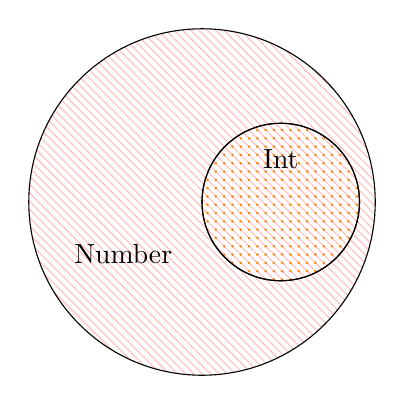
\begin{tikzpicture}
\usetikzlibrary{patterns}
  
\draw[pattern=north west lines, pattern color=pink] (0,0) circle (2.2);
\draw[pattern=dots, pattern color=orange
] (1,0) circle (1);
\draw (1,0.8)     node [text=black,below] {Int};
\draw (1,0) circle (1)  ;
\draw (-1.0,-0.4) node [text=black,below] {Number};
\end{tikzpicture}

}


  Failure to identify subtypes/supertypes will lead to \Emph{correct} but \Emph{inefficient} code.
\end{frame}




\begin{frame}{Rewrite: 3}
  \begin{columns}
    \begin{column}{0.5\textwidth}
      \colorbox{pink!30}{\code{(STop \& x)} $\to$ \code{x}}\\
      \colorbox{pink!30}{\code{!STop} $\to$ \code{SEmpty}}
      
      \usebox\typecaseCbox
    \end{column}
    \begin{column}{0.5\textwidth}  %%
      \colorbox{pink!30}{\code{(SEmpty \& x)} $\to$ \code{SEmpty}}\\
      \colorbox{pink!30}{\code{!SEmpty} $\to$ \code{STop}}

      \usebox\typecaseDhbox
    \end{column}    
  \end{columns}
\end{frame}

\begin{frame}{Rewrite: 4}
  \begin{columns}
    \begin{column}{0.5\textwidth}
      \colorbox{pink!30}{\code{SEmpty.typep(x)} $\to$ \code{false}}
      
      \usebox\typecaseDbox
    \end{column}
    \begin{column}{0.5\textwidth}  %%
      \colorbox{pink!30}{\code{STop.typep(x)} $\to$ \code{true}}

      \usebox\typecaseEhbox
    \end{column}    
  \end{columns}
\end{frame}

\begin{frame}{Rewrite: 5}
  \colorbox{pink!30}{\code{(if true x else y)} $\to$ \code{x}}\\
  \colorbox{pink!30}{\code{(if false x else y)} $\to$ \code{y}}

  \begin{columns}
    \begin{column}{0.5\textwidth}
      \usebox\typecaseEbox
    \end{column}
    \begin{column}{0.5\textwidth}  %%
      \usebox\typecaseFhbox
    \end{column}    
  \end{columns}
\end{frame}

\begin{frame}{Rewrite: 6}
  Introduce \colorbox{pink!30}{\code{if I.typep(x) ... else ...}}

  \begin{columns}
    \begin{column}{0.5\textwidth}
      \usebox\typecaseFbox
    \end{column}
    \begin{column}{0.5\textwidth}  %%
      \usebox\typecaseGabox
    \end{column}    
  \end{columns}
\end{frame}

\begin{frame}{Rewrite: 6}
  Introduce \colorbox{pink!30}{\code{if I.typep(x) ... else ...}}

  \begin{columns}
    \begin{column}{0.5\textwidth}
      \usebox\typecaseFbox
    \end{column}
    \begin{column}{0.5\textwidth}  %%
      \usebox\typecaseGbox
    \end{column}    
  \end{columns}
\end{frame}

\begin{frame}{Rewrite: 7}
  In \code{if} part: \colorbox{pink!30}{Supertypes of \code{I} $\to$ \code{STop}}\\
  In \code{else} part: \colorbox{pink!30}{Subtypes of \code{I} $\to$ \code{SEmpty}}

  \begin{columns}
    \begin{column}{0.5\textwidth}
      \usebox\typecaseGbox
    \end{column}
    \begin{column}{0.5\textwidth}  %%
      \usebox\typecaseHhbox
    \end{column}    
  \end{columns}
\end{frame}


\begin{frame}{Rewrite: 8}

  \begin{columns}
    \begin{column}{0.5\textwidth}
      \colorbox{pink!30}{\code{!STop} $\to$ \code{SEmpty}}
      \usebox\typecaseHbox
    \end{column}
    \begin{column}{0.5\textwidth}  %%
      \colorbox{pink!30}{\code{!SEmpty} $\to$ \code{STop}}
      \usebox\typecaseIhbox
    \end{column}    
  \end{columns}
\end{frame}

\begin{frame}{Rewrite: 9}

  \begin{columns}
    \begin{column}{0.5\textwidth}
      \colorbox{pink!30}{\code{SEmpty.typep(x)} $\to$ \code{false}}
      \usebox\typecaseIbox
    \end{column}
    \begin{column}{0.5\textwidth}  %%
      \colorbox{pink!30}{\code{STop.typep(x)} $\to$ \code{true}}
      \usebox\typecaseJhbox
    \end{column}    
  \end{columns}
\end{frame}

\begin{frame}{Rewrite: 10}
  \colorbox{pink!30}{\code{(if true x else y)} $\to$ \code{x}}\\
  \colorbox{pink!30}{\code{(if false x else y)} $\to$ \code{y}}

  \begin{columns}
    \begin{column}{0.5\textwidth}
      \usebox\typecaseJbox
    \end{column}
    \begin{column}{0.5\textwidth}  %%
      \usebox\typecaseKhbox
    \end{column}
  \end{columns}
\end{frame}


\begin{frame}{Rewrite: Summary}
  Code has been rewritten so that \Emph{any type check occurs no more than once}.

  \begin{columns}
    \begin{column}{0.5\textwidth}
      \usebox\typecaseAbox
    \end{column}
    \begin{column}{0.5\textwidth}  %%
      \usebox\typecaseKbox
    \end{column}
  \end{columns}

  And it is clear the the code never returns \code{None}.

\end{frame}

\begin{frame}{Decision Tree, Before and After}
  Viewing the \code{if ... else ...} before and after as decision trees.

  \begin{columns}
    \begin{column}{0.5\textwidth}
      \usebox\typecaseITEbox
    \end{column}
    \begin{column}{0.5\textwidth}  %%
      \usebox\typecaseITEafterbox
    \end{column}
  \end{columns}
\end{frame}




